
\documentclass{article}
\usepackage{polski}
\usepackage[utf8]{inputenc}
\usepackage{enumerate}
\usepackage{blindtext}
\usepackage{graphicx}
\usepackage{geometry}
\usepackage{listings}
\usepackage{float}
\usepackage[table]{xcolor}
\setlength{\parskip}{0pt} 
\newgeometry{lmargin = 3cm, rmargin=2.5cm}
\renewcommand{\labelenumi}{\arabic{enumi}.}
\renewcommand{\labelenumii}{\arabic{enumi}.\arabic{enumii}.}


\begin{document}
\begin{titlepage}
	\centering
	
\includegraphics[width=0.15\textwidth]{agh}\par\vspace{1cm}	
	{\scshape\large AKADEMIA GÓRNICZO-HUTNICZA \\IM. STANISŁAWA STASZICA W KRAKOWIE \par}
	\vspace{0.5cm}
	{\scshape\large Wydział elektrotechniki automatyki	informatyki i inżynierii biomedycznej \par}
	\vspace{0.5cm}
	{\scshape\Large Informatyka \par}
	\vspace{1cm}
	{\huge\bfseries Wykorzystanie SAT Solverów w tworzeniu grafików\par}
	\vspace{2cm}
	{\large Izabela Kiełbasa \\ Natalia Janecka\par}
	\vfill
	\vfill
	{\large \today\par}
\end{titlepage}
%%\tableofcontents
\clearpage
\section{Użycie SAT Solvera w projekcie}
\par
Do rozwiązywania problemów SAT w projekcie została wykorzystana biblioteka dla Javy: \textbf{Sat4j}. Umożliwia ona rozwiązywanie problemów satysfakcji zdań logicznych oraz optymalizacji. Pozwala na rozwiązanie problemów SAT, MAXSAT, Pseudo-Boolean oraz Minimally Unsatisfable Subset (MUS). \\
Biblioteka ta jest przyjazna dla użytkownika i zaprojektowana elastycznie używając wzorców projektowych takich jak dekorator i strategia. Jej zaletą jest również to, że jest open source. \\ \\
SAT przyjmuje zdanie logoczne w formie \textbf{CNF} – koniunkcyjna postać normalna. Formuła zapisana w koniunkcji klauzul np.: $$ (x1 \vee x2 \vee x3) \wedge (x4 \vee x2) $$
Każda formuła CNF składa się ze \textbf{zmiennych}, które mogą przyjmować tylko wartości \textbf{\textit{prawda}} lub \textbf{\textit{fałsz}} (dla powyższego przykładu jest ich 4) oraz \textbf{klauzul} na zmiennych np.: $$ C1\wedge C2\wedge ...\wedge Cn $$(dla powyższego przykładu mamy 2 klauzule). \\ \\
SAT znajduje rozwiązanie dla podanego zdania tak aby cała formuła była prawdziwa (wszystkie klauzule muszą być prawdziwe). Jeśli rozwiązanie nie istnieje to SAT zwraca odpowiednią informację. \\
MAXSAT znajduje jak najwięszką ilość zmiennych tak aby zdanie było prawdziwe. Natomiast MUS znajduje jak najmiejszą ilość zmiennych dla której zdanie jest niespełnione. \\ \\
\par
Bibioteka sat4j przyjmuje jako wejście plik o rozszerzeniu \textbf{.cnf}. Plik ten składa się z 2 części:\textit{ preambuły} oraz \textit{klauzul}. 
\begin{enumerate}
\item \underline{Preambuła} zawiera informacje na temat przykładu. Każda linia zaczyna się od litery która ją charakteryzuje. 
\begin{itemize}
	\item Linia komentarza zaczyna się od litery “c” a po niej nastepuje spacja i komentarz
	\item 
 Problem line – jedna linia dla pliku, definiuje zawartość pliku. Dla pliku CNF wygląda ona natępująco:
\begin{lstlisting}
p cnf iloscZmiennych iloscKlauzul 
\end{lstlisting} 
\end{itemize} 
\item
Druga część pliku to \underline{część klauzul} – pojawia się ona bezpośrednio po linii problemu. Zmienne są ponumerowane od 1 do n (gdzie n to ilość zmiennych). Każda klauzula jest reprezentowana jako sekwencja liczb, oddzielonych od siebie spacją, tabem lub znakiem nowej linii. Zmienna prawdziwa jest zapisywana jako $i$,  a zmienna fałszywa jako $\neg i$. Każda klauzula jest zakończona wartością 0. 
Dla powyzszego przykładu plik .cnf ma postać
\begin{lstlisting}
	p cnf 4 2
	1 2 3 0
	4 2 0
\end{lstlisting}

Jako rozwiązanie SATa będzie tu przedstawiona linia
\begin{lstlisting}
1 2 3 4 0
\end{lstlisting}

co oznacza, że aby dana formuła była prawdziwa wszystkie jej zmienne muszą być prawdziwe.  Jeśli przed którąś ze zmiennych byłby znak "$\neg$" to zmienna ta powinna być fałszywa aby formuła była spełniona. 
\end{enumerate}


\section{Słownik pojęć}
\par
\begin{itemize}
	\item Instruktor - osoba pracująca, która prowadzi jazdy, ma określone godziny pracy(patrz niżej), jednocześnie może prowadzić zajęcia tylko z jednym kursantem
	\item kursant - osoba uczestnicząca w zajęciach, może wybrać jednego instruktora z listy, z którym chce odbywać jazdy. Ma określone preferowane godziny zajęć(patrz niżej). Osteczna godzina zajęć zostanie wybrana z listy preferowanych przez kursanta jeśli wybrany przez niego instruktor jest wtedy dostępny  
	\item Godziny pracy instruktora - para liczb: godzina rozpoczęcia pracy i godzina zakończenia pracy. Pierwsza liczba zawsze musi być mniejsza od drugiej. Może być kilka takich par - oznacza to, że instruktor pracuje z przerwami w godzinach, które nie zawierają sie pomiędzy liczbami w parach.
	\item Preferowane godziny zajęć - pary liczb - godzina rozpoczęcia i zakończenia jazdy. W tym czasie kursant może odbywać jazdy. Może być ich kilka

\end{itemize}
\section{Tworzenie grafiku}
\par
W aplikacji możemy dodać instruktorów i wybrać dla nich godziny pracy. \\ \\ 

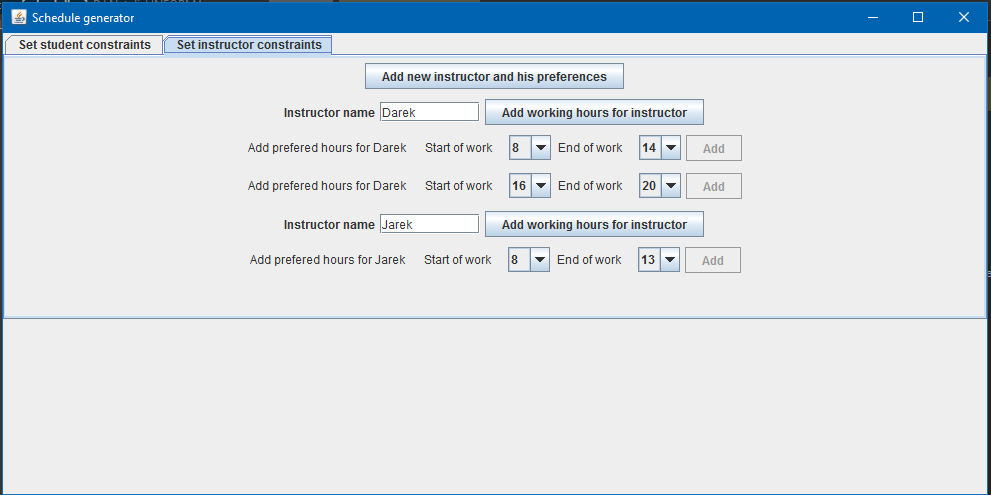
\includegraphics[width=0.5\textwidth]{screen-instuktorzy.png} \\ \\
W drugiej zakładce można dodać kursantów. Wybieramy dla każdego jednego instruktora oraz godziny, w których chciałby mieć zajęcia. \\ \\

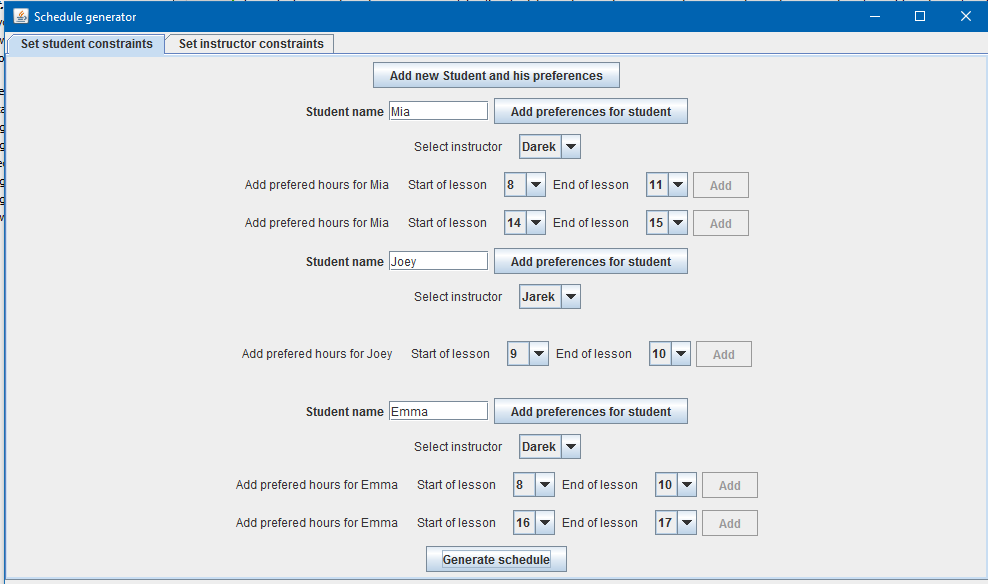
\includegraphics[width=0.5\textwidth]{screen-kursanci.png} \\ \\
Kiedy dodaliśmy już wszystkie preferencje klikamy przycisk $Generate$. W nowym okienku pokaże nam się wygenerowany przez SAT grafik, który spełnia wszystkie ograniczenia. \\ Wynikowa tabelka jest posortowana według instruktorów, a następnie godzin rozpoczęcia jazdy. \\ \\
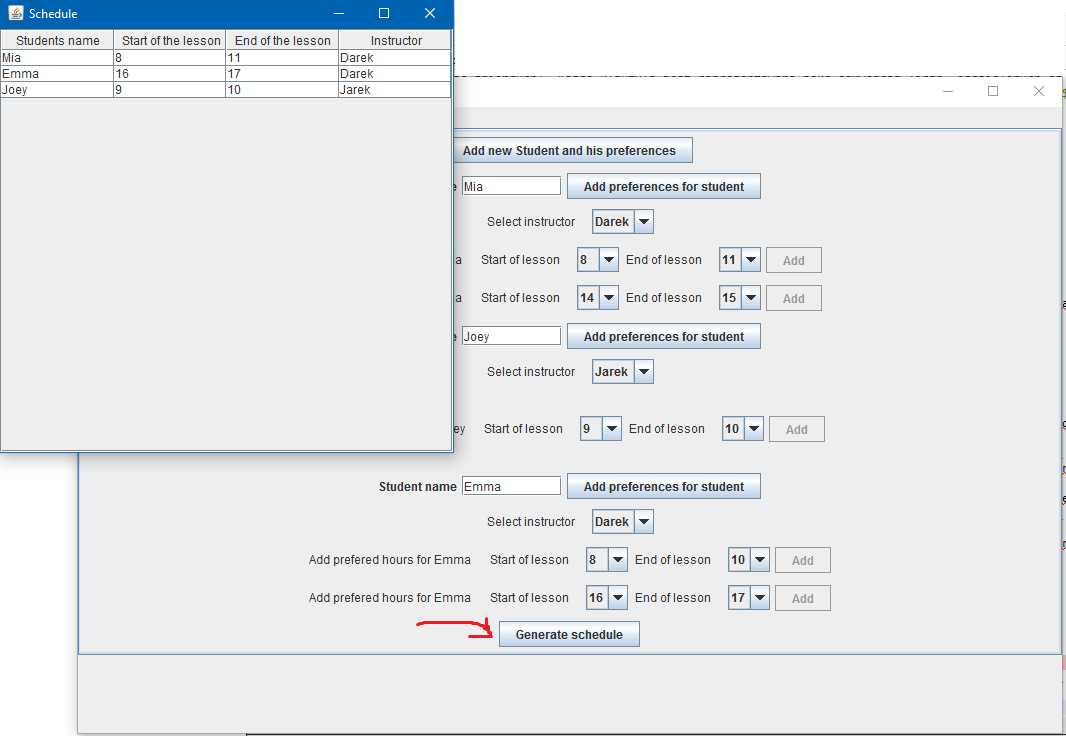
\includegraphics[width=0.5\textwidth]{screen-final.png}
\end{document}